\subsection{Funktionsweise} \label{sec:funktionsweise}

Der Dojo ist eine Art Audio-Guide welcher für Museen designt ist und diverse Funktionen beinhaltet. Abbildung \ref{fig:Funktion Dojo} visualisiert den von der Auftraggeberin designten Prototypen. Einer der grössten Abweichungen zu einem herkömmlichen Audio-Guide ist die Sprachausgabe mittels einem Köperschallaktor und nicht wie gewöhlich einem Lautsprecher. Eine der Eigenheiten ist ein integrierter Like Button, mit dem man Ausstellungsstücke \glqq liken \grqq kann. Diese Likes können am Ende des Museumsbesuchs zusammengefasst und in einer nicht genauer definierten Form an den Besucher abgegeben. Ansonsten kann der Dojo das was man von einem Audio-Guide erwarten würde, wie der Audiowiedergabe, Haltemodus und Lautstärke Einstellung.

\begin{figure}[H]
	\begin{center}
		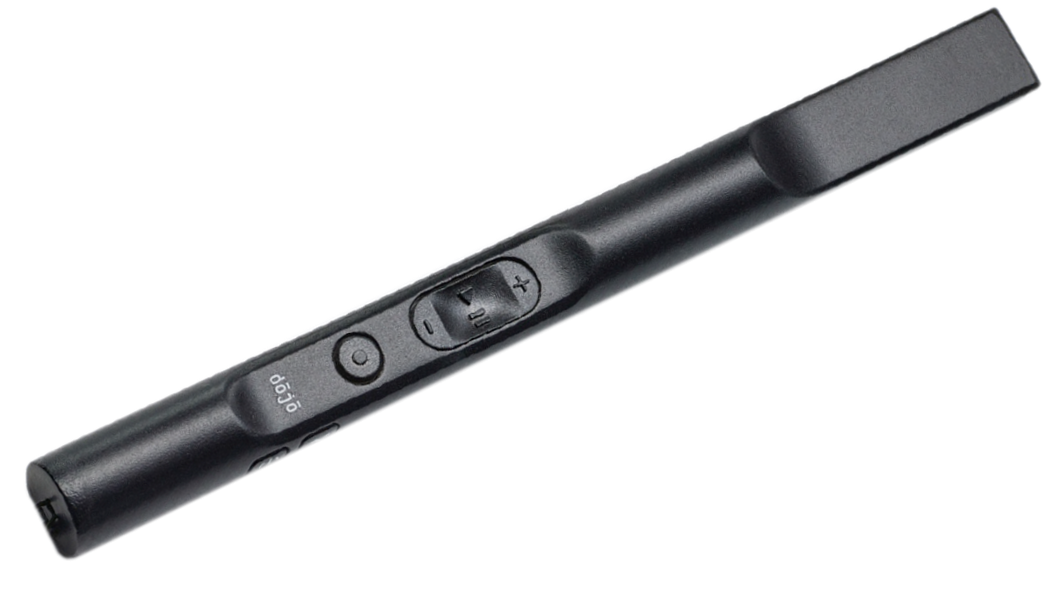
\includegraphics[width=140mm]{data/Dojo.png}
		\caption[Dojo als Modell]{Dojo als Modell} %picture caption
		\label{fig:Funktion Dojo}
	\end{center}
\end{figure}

Das Herzstück des Dojo ist ein NRF52 von Nordic Semiconductor mit integriertem Bluetooth-Stack, welcher wiederum low-Energy fähig ist. Die Daten werden auf einer SD-Karte gespeichert. Einen Überblick über die Teilsysteme des Dojos ergibt Abbildung \ref{fig:Teilsysteme}. Der NRF52 wird die Audiodaten an den Verstärker weitergeben, welcher sie über den Körperschallaktor ausgibt. Gespeist wird der Dojo von einem Akku, welcher induktiv geladen wird.

\begin{figure}[H]
	\begin{center}
		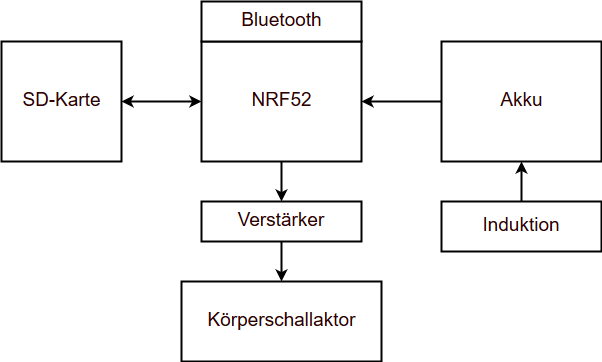
\includegraphics[width=110mm]{data/Loesungskonzept_Teilsysteme.png}
		\caption{Teilsysteme des Dojo} %picture caption
		\label{fig:Teilsysteme}
	\end{center}
\end{figure}

Die Funktion des Dojos sind in zwei Bereiche unterteilt. Im Abschnitt \nameref{sec:funktionNutzer} sind die Funktionen für die Museumsbesucher beschrieben, welche nachfolgend als User bezeichnet werden. Zum anderen sind im Abschnitt \nameref{sec:funktionBetreiber} die für die Museumsbetreiber relevanten Funktionen beschrieben. Diese werden nachfolgend als Betreiber bezeichnet.

\subsubsection*{Nutzer} \label{sec:funktionNutzer}
Der User geht mit dem Dojo durch das Museum. Sobald die Bluetooth Beacons genug nahe sind, wird dem Nutzer ein Signal gesendet. Dies erfolgt durch Vibration oder mithilfe einer LED. Jetzt soll der User entscheiden ob er sich das zugehörige Audio-File anhören will. Will er das, kann er den Play-Button betätigen. Die Lautstärke kann über die Buttons justiert werden. Falls das Ausstellungsstück dem Nutzer gefallen hat, kann er die Merken-Taste betätigen. Diese speichert das Ausstellungsstück auf eine Liste im Dojo. Am Ende des Museumsbesuches kann diese Liste ausgewertet werden, wobei die Anwendung dieser Daten in dieser Arbeit nicht weiter verfolgt wurden.

\subsubsection*{Betreiber} \label{sec:funktionBetreiber}
Der Betreiber muss den Dojo konfigurieren. Dies erfolgt über eine SD-Karte, welche mit dem Computer beladen wird. Anschliessend wird diese in den Dojo eingeführt. Das Nachladen des Akkumulator erfolgt über eine induktive Ladung. Die nächsten zwei Funktionen sind Wunschziele, die vor allem mit Rücksicht auf die Laufzeit realisiert werden. Den Bluetooth-Receiver könnte man kurzzeitig auf ein Bluetooth Beacon umschalten. Der Betreiber müsste nur noch einen Receiver pro Raum installieren. Damit könnte man die gewünschte HeatMap realisieren. Das zweite wäre die Möglichkeit per Bluetooth einzelne Audiofiles auf den Dojo zu übertragen, um im Falle einer Änderung der Austellung die Liste anzupassen.
